\documentclass[12pt,a4paper]{article}
\usepackage{amsmath,amsthm,amssymb,mathtools}
\usepackage{tikz}
\usetikzlibrary{arrows.meta,positioning,shapes.geometric,calc,fit,backgrounds}
\usepackage{graphicx}
\usepackage{booktabs,tabularx,multirow}
\usepackage[ruled,vlined,linesnumbered]{algorithm2e}
\usepackage[most]{tcolorbox}
\usepackage{hyperref}
\usepackage[capitalize,noabbrev]{cleveref}
\usepackage[margin=1in]{geometry}
\usepackage{fancyhdr}
\usepackage{enumitem}
\usepackage{xcolor}
\newtcolorbox{keyinsight}[1][]{colback=blue!5!white,colframe=blue!75!black,fonttitle=\bfseries,title=Key Insight,#1}
\newtcolorbox{example}[1][]{colback=green!5!white,colframe=green!75!black,fonttitle=\bfseries,title=Example,#1}
\newtcolorbox{warningbox}[1][]{colback=red!5!white,colframe=red!75!black,fonttitle=\bfseries,title=Warning,#1}
\newtheorem{theorem}{Theorem}[section]
\newtheorem{lemma}[theorem]{Lemma}
\newtheorem{definition}{Definition}[section]
\newtheorem{remark}{Remark}[section]

% Header/footer setup
\pagestyle{fancy}
\fancyhf{}
\rhead{Deep Learning -- Session 21}
\lhead{GRU \& Seq2Seq}
\rfoot{\thepage}

\hypersetup{
  colorlinks=true,
  linkcolor=blue!70!black,
  urlcolor=blue!70!black
}

\title{\textbf{Session 21: Gated Recurrent Unit (GRU) and\\
Sequence-to-Sequence Models}\\[0.5em]
\large Deep Learning Course\\
\normalsize IIT Dharwad -- Prof.\ S.\ R.\ M.\ Prasanna \& Dr.\ Sunil Saumya}
\author{Course Notes}
\date{February 2, 2026}

\begin{document}

\maketitle
\thispagestyle{fancy}

\begin{abstract}
These notes cover Session~21 of the deep learning course, which provides a thorough treatment of the
\textbf{Gated Recurrent Unit (GRU)}: its motivation as a simplified alternative to LSTM, the intuition
behind its two gates (reset gate $r_t$ and update gate $z_t$), its complete mathematical formulation,
a four-step numerical walkthrough, and a comparison with vanilla RNN and LSTM. The session concludes
with an introduction to the \textbf{Sequence-to-Sequence (Seq2Seq)} language model -- the foundational
architecture behind modern large language models (LLMs) -- including the encoder--decoder structure
and the role of the context vector.
\end{abstract}

\tableofcontents
\newpage

%=============================================================
\section{Introduction}
\label{sec:intro}
%=============================================================

Recurrent neural networks (RNNs) process sequential data by maintaining a hidden state that summarises
the history of the sequence seen so far.  Vanilla RNNs suffer from the \emph{vanishing/exploding
gradient} problem, which makes it difficult to capture long-range dependencies.  Long Short-Term Memory
(LSTM) networks address this limitation using a cell state $C_t$ and three learnable gates (forget,
input, output), but at the cost of a significantly higher parameter count.

The \textbf{Gated Recurrent Unit (GRU)}, proposed by Cho et al.\ (2014), offers a structurally simpler
alternative: it retains only \emph{one state line} $h_t$ (merging the separate cell state and hidden
state of LSTM) and uses \emph{two gates} instead of three.  This reduces memory and computation while
empirically matching LSTM performance on most benchmark tasks.

Session~21 also introduces the \textbf{Seq2Seq} architecture, which pairs an LSTM encoder with an LSTM
decoder connected via a fixed-size \emph{context vector}, forming the backbone of neural machine
translation and text summarisation systems.

\subsection{Learning Objectives}

After studying these notes the reader should be able to:
\begin{enumerate}[label=\arabic*.]
  \item Explain the architectural differences between RNN, LSTM, and GRU.
  \item Derive the four GRU equations from first principles.
  \item Perform a step-by-step numerical forward pass through a GRU cell.
  \item Identify how GRU gates correspond to LSTM gates.
  \item Describe the Seq2Seq encoder--decoder pipeline and its limitations.
\end{enumerate}

%=============================================================
\section{Background: From RNN to LSTM to GRU}
\label{sec:background}
%=============================================================

\subsection{Vanilla RNN Limitations}

A vanilla RNN maintains a single hidden state $h_t \in \mathbb{R}^d$ updated at each time step:
\begin{equation}
  h_t = \tanh\!\bigl(W_h\,h_{t-1} + W_x\,x_t + b\bigr).
  \label{eq:rnn}
\end{equation}
During back-propagation through time (BPTT) the gradient must pass through a chain of weight matrices.
When $\|W_h\| < 1$ the gradient vanishes; when $\|W_h\| > 1$ it explodes. In practice, dependencies
beyond 10--20 time steps are poorly captured.

\subsection{LSTM: Gating to Preserve Long-Term Context}

LSTM introduces a \emph{cell state} $C_t$ (long-term memory) alongside a hidden state $h_t$
(short-term memory) and three sigmoid gates:
\begin{align}
  f_t &= \sigma(W_f [h_{t-1}, x_t] + b_f), \label{eq:lstm_forget}\\
  i_t &= \sigma(W_i [h_{t-1}, x_t] + b_i), \label{eq:lstm_input}\\
  o_t &= \sigma(W_o [h_{t-1}, x_t] + b_o), \label{eq:lstm_output}\\
  \tilde{C}_t &= \tanh(W_C [h_{t-1}, x_t] + b_C), \label{eq:lstm_candidate}\\
  C_t &= f_t \odot C_{t-1} + i_t \odot \tilde{C}_t, \label{eq:lstm_cell}\\
  h_t &= o_t \odot \tanh(C_t). \label{eq:lstm_hidden}
\end{align}
The additive cell-state update in \cref{eq:lstm_cell} provides a gradient highway that alleviates
vanishing gradients. However, LSTM requires \emph{four} weight matrices (one per sub-network) and
\emph{two} parallel state lines, increasing both parameter count and memory footprint.

\begin{keyinsight}[title=LSTM State Summary]
LSTM uses \textbf{2 states} ($h_t$, $C_t$) and \textbf{3 gates} ($f$, $i$, $o$).
The cell state carries long-term context (LTC) and the hidden state carries short-term context (STC).
\end{keyinsight}

\subsection{Historical Note}

Interestingly, from a historical perspective the GRU was proposed \emph{before} LSTM became dominant.
As explained by Prof.\ Prasanna in Session~21:

\begin{quote}
``Initially RNN was there. When they found there is a problem in modelling the long-term context
information, they proposed GRU first, and then they segregated into LSTM. But LSTM became so prevalent
that now we study LSTM first.''
\end{quote}

%=============================================================
\section{Gated Recurrent Unit: Architecture}
\label{sec:gru_arch}
%=============================================================

\subsection{Structural Overview}

The GRU reduces LSTM complexity in two ways:
\begin{enumerate}
  \item \textbf{One state line}: $h_t$ carries both short-term context (STC) and long-term context
        (LTC) information simultaneously, with different dimensions of the vector specialised for each.
  \item \textbf{Two gates}: the reset gate $r_t$ and the update gate $z_t$ together replicate the
        combined function of LSTM's three gates.
\end{enumerate}

\cref{tab:rnn_comparison} summarises the architectural comparison.

\begin{table}[htbp]
\centering
\caption{Structural comparison of RNN, LSTM, and GRU.}
\label{tab:rnn_comparison}
\begin{tabular}{@{}lccc@{}}
\toprule
\textbf{Feature} & \textbf{RNN} & \textbf{LSTM} & \textbf{GRU} \\
\midrule
States & 1 ($h_t$) & 2 ($h_t$, $C_t$) & 1 ($h_t$) \\
Gates & 0 & 3 ($f$, $i$, $o$) & 2 ($r$, $z$) \\
Sub-networks & 1 & 4 & 3 \\
LTC / STC lines & Single (STC only) & Separate & Unified \\
Parameters & Fewest & Most & Moderate \\
Training speed & Fastest & Slowest & Intermediate \\
\bottomrule
\end{tabular}
\end{table}

\begin{keyinsight}[title=GRU Design Philosophy]
GRU merges $h_t$ and $C_t$ into a single vector. Some dimensions of $h_t$ specialise in
long-term context, while others carry short-term context. The reset and update gates
determine \emph{which dimensions are updated} at each time step.
\end{keyinsight}

\subsection{TikZ Diagram: GRU Cell}

\begin{figure}[htbp]
\centering
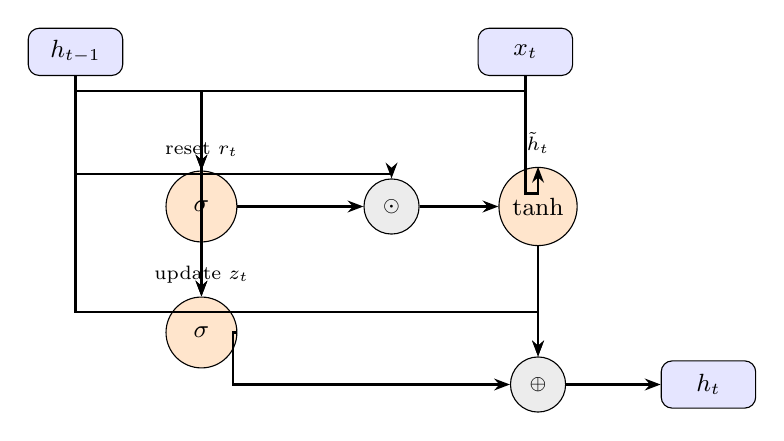
\begin{tikzpicture}[
  node distance=1.4cm and 2.0cm,
  gate/.style={draw,circle,minimum size=0.9cm,fill=orange!20,font=\small},
  op/.style={draw,circle,minimum size=0.7cm,fill=gray!15,font=\scriptsize},
  state/.style={draw,rectangle,rounded corners,minimum width=1.2cm,minimum height=0.6cm,
                fill=blue!10,font=\small},
  arr/.style={-{Stealth[length=2mm]},thick},
  every label/.style={font=\scriptsize}
]

% Inputs
\node[state] (ht1) {$h_{t-1}$};
\node[state, right=4.5cm of ht1] (xt) {$x_t$};

% Reset gate
\node[gate, below=1.2cm of ht1, xshift=1.6cm] (rgate) {$\sigma$};
\node[font=\scriptsize, above=0.05cm of rgate] {reset $r_t$};

% Update gate
\node[gate, below=2.8cm of ht1, xshift=1.6cm] (zgate) {$\sigma$};
\node[font=\scriptsize, above=0.05cm of zgate] {update $z_t$};

% Hadamard product reset * h_{t-1}
\node[op, right=1.6cm of rgate] (hadR) {$\odot$};

% Candidate tanh
\node[gate, right=1.0cm of hadR] (tanh1) {tanh};
\node[font=\scriptsize, above=0.05cm of tanh1] {$\tilde{h}_t$};

% Final blend
\node[op, below=1.4cm of tanh1] (blend) {$\oplus$};

% Output
\node[state, right=1.2cm of blend] (ht) {$h_t$};

% Arrows
\draw[arr] (ht1) -- ++(0,-0.5) -| (rgate);
\draw[arr] (xt) -- ++(0,-0.5) -| (rgate);
\draw[arr] (ht1) -- ++(0,-0.5) -| (zgate);
\draw[arr] (xt) -- ++(0,-0.5) -| (zgate);
\draw[arr] (rgate) -- (hadR);
\draw[arr] (ht1) -- ++(0,-1.55) -| (hadR);
\draw[arr] (hadR) -- (tanh1);
\draw[arr] (xt) -- ++(0,-1.8) -| (tanh1);
\draw[arr] (tanh1) -- ++(0,-0.65) -- (blend);
\draw[arr] (zgate) -- ++(0.4,0) |- (blend);
\draw[arr] (ht1) -- ++(0,-3.3) -| (blend);
\draw[arr] (blend) -- (ht);

\end{tikzpicture}
\caption{Simplified GRU cell.  The reset gate $r_t$ controls how much of the previous hidden state
feeds into the candidate; the update gate $z_t$ performs linear interpolation between the old state
and the candidate.}
\label{fig:gru_cell}
\end{figure}

%=============================================================
\section{GRU: Intuition and Notation}
\label{sec:gru_intuition}
%=============================================================

\subsection{Motivating Example: Reading a Paragraph}

\begin{example}[title=Sequential Memory in Text]
Consider the following paragraph processed token by token:
\begin{quote}
``Generative AI can generate new content. Generative AI is a type of Deep Learning.
Deep Learning is a subset of Neural Networks. Neural Networks are part of Machine Learning.''
\end{quote}
\begin{itemize}[noitemsep]
  \item When reading \emph{Generative AI} in sentence 2, the term already exists in memory -- no
        new information is needed for that token.
  \item When reading \emph{Deep Learning} for the first time, this is new information and should
        be added to memory.
  \item The word \emph{Deep Learning} reappears in sentence 3; the model may choose not to add
        it again.
  \item \emph{Neural Networks} and \emph{Machine Learning} carry new relational information.
\end{itemize}
The GRU decides at each time step: \textbf{what to remember, what to forget, and what new information
to add} -- exactly the same goal as LSTM, but with fewer parameters.
\end{example}

\subsection{Variable Notation}

\cref{tab:gru_notation} lists all variables used in the GRU formulation.

\begin{table}[htbp]
\centering
\caption{GRU variable notation at time step $t$.}
\label{tab:gru_notation}
\begin{tabular}{@{}clc@{}}
\toprule
\textbf{Symbol} & \textbf{Description} & \textbf{Range / Shape} \\
\midrule
$x_t$ & Input vector at time $t$ & $x_t \in \mathbb{R}^k$ \\
$h_{t-1}$ & Previous hidden state (memory) & $h_{t-1} \in \mathbb{R}^d$ \\
$r_t$ & Reset gate output & $r_t \in (0,1)^d$ \\
$z_t$ & Update gate output & $z_t \in (0,1)^d$ \\
$\tilde{h}_t$ & Candidate hidden state & $\tilde{h}_t \in (-1,1)^d$ \\
$h_t$ & Final hidden state & $h_t \in \mathbb{R}^d$ \\
$W_r, W_z, W$ & Learned weight matrices & $\mathbb{R}^{d \times (d+k)}$ \\
\bottomrule
\end{tabular}
\end{table}

\begin{remark}
All internal vectors $r_t$, $z_t$, $\tilde{h}_t$, and $h_t$ share the same dimension $d$,
determined by the chosen hidden size. Only $x_t$ may have a different dimension $k$.
This uniform dimensionality is required for the element-wise (Hadamard) products $\odot$.
\end{remark}

\subsection{Two-Stage Memory Update}

The GRU updates memory in exactly two stages:
\begin{equation}
  h_{t-1} \;\longrightarrow\; \tilde{h}_t \;\longrightarrow\; h_t.
  \label{eq:two_stage}
\end{equation}
Stage~1 (computing $\tilde{h}_t$) uses the \emph{reset gate} to decide how much of the old state to
``reset'' before computing a candidate. Stage~2 (computing $h_t$) uses the \emph{update gate} to
linearly interpolate between the old state and the candidate.

\begin{keyinsight}[title=Two-Stage Analogy]
Think of watching a mystery film: $h_{t-1}$ is your current belief about the plot. When a new scene
arrives ($x_t$), you first \emph{reassess} your old belief with the reset gate (perhaps forgetting
some assumptions) and form a candidate new belief $\tilde{h}_t$. Then you \emph{balance} your old
belief with the candidate via the update gate to arrive at $h_t$. You cannot rely 100\% on the
new candidate because future plot twists may reverse it.
\end{keyinsight}

%=============================================================
\section{GRU Mathematical Formulation}
\label{sec:gru_math}
%=============================================================

\subsection{The Four Core Equations}

Let $[\,h_{t-1},\,x_t\,]$ denote the concatenation of the previous hidden state and the current
input. The GRU forward pass is defined by:

\begin{align}
  z_t &= \sigma\!\bigl(W_z\cdot[h_{t-1},\,x_t]\bigr),
  \label{eq:update_gate} \\[4pt]
  r_t &= \sigma\!\bigl(W_r\cdot[h_{t-1},\,x_t]\bigr),
  \label{eq:reset_gate} \\[4pt]
  \tilde{h}_t &= \tanh\!\bigl(W\cdot[r_t \odot h_{t-1},\,x_t]\bigr),
  \label{eq:candidate} \\[4pt]
  h_t &= (1 - z_t)\odot h_{t-1} \;+\; z_t\odot\tilde{h}_t.
  \label{eq:hidden_update}
\end{align}

\cref{eq:update_gate,eq:reset_gate} each correspond to a single-layer neural network with a sigmoid
activation. They share the same input $[h_{t-1}, x_t]$ but have \emph{distinct} weight matrices
$W_z$ and $W_r$ -- this is why their outputs $z_t$ and $r_t$ differ.

\cref{eq:candidate} computes the candidate hidden state by first masking the previous hidden state
with the reset gate ($r_t \odot h_{t-1}$) before concatenating with $x_t$ and passing through
$\tanh$.

\cref{eq:hidden_update} performs a convex combination: when $z_t \approx 1$ the output is
dominated by the new candidate; when $z_t \approx 0$ the old state is preserved.

\subsection{Gate Correspondence with LSTM}

\begin{table}[htbp]
\centering
\caption{Functional mapping between GRU and LSTM gates.}
\label{tab:gate_map}
\begin{tabular}{@{}lll@{}}
\toprule
\textbf{GRU component} & \textbf{LSTM equivalent} & \textbf{Function} \\
\midrule
Reset gate $r_t$ & Forget gate $f_t$ & Selectively erase old memory \\
$(1 - z_t)$ & Input gate $i_t$ & Control new information added \\
Update gate $z_t$ & Output gate $o_t$ & Control how much to expose \\
Single state $h_t$ & Cell state $C_t$ + hidden $h_t$ & Unified LTC + STC storage \\
\bottomrule
\end{tabular}
\end{table}

\begin{warningbox}[title=Common Misconception]
The GRU does \textbf{not} simply drop one LSTM gate and keep the rest unchanged.  The update gate
$z_t$ simultaneously plays the role of the LSTM output gate, while $(1-z_t)$ acts as the input gate.
The input gate is \emph{derived} from the update gate rather than being an independent learnable
network, which is the core structural simplification.
\end{warningbox}

\subsection{Data Flow Diagram}

\begin{figure}[htbp]
\centering
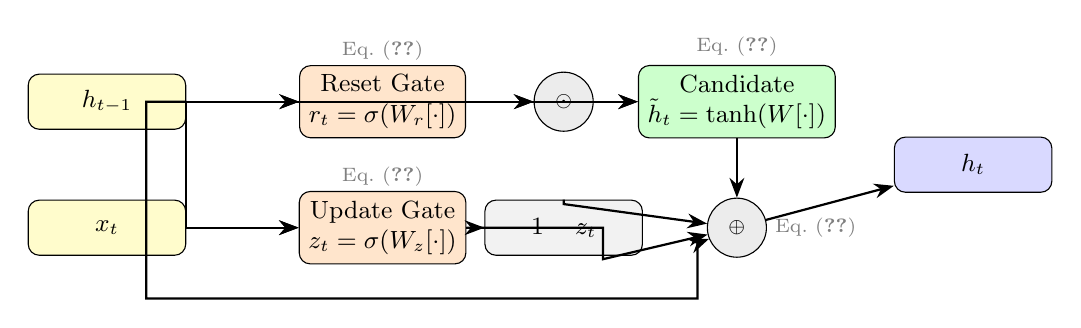
\begin{tikzpicture}[
  box/.style={draw,rounded corners,minimum width=2.0cm,minimum height=0.7cm,
              fill=yellow!20,font=\small,align=center},
  op/.style={draw,circle,minimum size=0.75cm,fill=gray!15,font=\scriptsize},
  arr/.style={-{Stealth[length=2.5mm]},thick},
  label style/.style={font=\scriptsize\itshape}
]

\node[box] (ht1)  at (0,0)   {$h_{t-1}$};
\node[box] (xt)   at (0,-1.6) {$x_t$};

% Reset gate block
\node[box,fill=orange!20] (rblock) at (3.5,0) {Reset Gate\\$r_t = \sigma(W_r[\cdot])$};
% Hadamard
\node[op] (had) at (5.8,0) {$\odot$};
% tanh
\node[box,fill=green!20] (tanhb) at (8.0,0) {Candidate\\$\tilde{h}_t = \tanh(W[\cdot])$};

% Update gate block
\node[box,fill=orange!20] (zblock) at (3.5,-1.6) {Update Gate\\$z_t = \sigma(W_z[\cdot])$};
% Blend
\node[op] (blend) at (8.0,-1.6) {$\oplus$};
% Output
\node[box,fill=blue!15] (ht) at (11.0,-0.8) {$h_t$};

% 1-z
\node[box,fill=gray!10] (onez) at (5.8,-1.6) {$1-z_t$};

% Arrows
\draw[arr] (ht1) -- (rblock);
\draw[arr] (xt) -- ++(1.0,0) |- (rblock);
\draw[arr] (rblock) -- (had);
\draw[arr] (ht1) -- ++(2.2,0) -- (had);
\draw[arr] (had) -- (tanhb);
\draw[arr] (xt) -- ++(1.0,0) |- (tanhb);
\draw[arr] (tanhb) -- ++(0,-0.5) -- (blend);

\draw[arr] (ht1) -- ++(1.0,0) |- (zblock);
\draw[arr] (xt) -- (zblock);
\draw[arr] (zblock) -- (onez);
\draw[arr] (onez) -- ++(0,0.3) -- (blend);
\draw[arr] (zblock) -- ++(2.8,0) -- ++(0,-0.4) -- (blend);
\draw[arr] (ht1) -- ++(0.5,0) -- ++(0,-2.5) -- ++(7.0,0) -- ++(0,0.7) -- (blend);
\draw[arr] (blend) -- (ht);

\node[font=\scriptsize,color=gray] at (8.0,0.7) {Eq.~(\ref*{eq:candidate})};
\node[font=\scriptsize,color=gray] at (3.5,0.65) {Eq.~(\ref*{eq:reset_gate})};
\node[font=\scriptsize,color=gray] at (3.5,-0.95) {Eq.~(\ref*{eq:update_gate})};
\node[font=\scriptsize,color=gray] at (9.0,-1.6) {Eq.~(\ref*{eq:hidden_update})};

\end{tikzpicture}
\caption{GRU data-flow diagram illustrating all four equations.  Signals from $h_{t-1}$ and $x_t$
feed both gates; the reset gate first masks $h_{t-1}$ before computing the candidate;
the update gate performs the final convex combination.}
\label{fig:gru_dataflow}
\end{figure}

\subsection{Gradient Flow Properties}

The linear interpolation in \cref{eq:hidden_update} provides an additive path for gradients:
\begin{equation}
  \frac{\partial h_t}{\partial h_{t-1}} = (1-z_t) + z_t\,\frac{\partial\tilde{h}_t}{\partial h_{t-1}}.
\end{equation}
The term $(1-z_t)$ is a direct gradient path -- analogous to the cell-state highway in LSTM --
that allows gradients to flow without being multiplied by potentially small values, thereby
mitigating vanishing gradients.

\begin{keyinsight}[title=Update Gate as Interpolation]
When $z_t = 1$, the output is entirely the new candidate $\tilde{h}_t$; when $z_t = 0$, the
output is entirely the old state $h_{t-1}$. The smooth blending prevents abrupt state overwrites
and enables stable gradient flow over long sequences.
\end{keyinsight}

%=============================================================
\section{Numerical Walkthrough}
\label{sec:numerical}
%=============================================================

This section performs a complete 4-step GRU forward pass on a concrete numerical example with
$d = 4$ (hidden dimension).

\subsection{Given Values}

\begin{align}
  h_{t-1} &= \begin{bmatrix} 0.4 \\ 0.3 \\ -0.2 \\ 0.1 \end{bmatrix},
  \quad
  x_t = \begin{bmatrix} 0.8 \\ -0.1 \\ 0.5 \\ 0.2 \end{bmatrix}.
\end{align}

\subsection{Step 1: Update Gate $z_t$}

\begin{equation}
  z_t = \sigma(W_z\cdot[h_{t-1},\,x_t])
  \;\Longrightarrow\;
  z_t = \begin{bmatrix} 0.89 \\ 0.58 \\ 0.96 \\ 0.90 \end{bmatrix}.
\end{equation}
Each element is between 0 and 1 because of the sigmoid activation.

\subsection{Step 2: Reset Gate $r_t$}

\begin{equation}
  r_t = \sigma(W_r\cdot[h_{t-1},\,x_t])
  \;\Longrightarrow\;
  r_t = \begin{bmatrix} 0.64 \\ 0.49 \\ 0.15 \\ 0.84 \end{bmatrix}.
\end{equation}
Elements close to~0 cause the corresponding dimensions of $h_{t-1}$ to be heavily suppressed,
effectively ``resetting'' those memory slots.

\subsection{Step 3: Candidate Hidden State $\tilde{h}_t$}

\begin{equation}
  \tilde{h}_t = \tanh(W\cdot[r_t\odot h_{t-1},\,x_t])
  \;\Longrightarrow\;
  \tilde{h}_t = \begin{bmatrix} 0.38 \\ 0.55 \\ -0.26 \\ 0.64 \end{bmatrix}.
\end{equation}
The $\tanh$ activation squashes values to $(-1, 1)$.

\subsection{Step 4: Final Hidden State $h_t$}

Applying \cref{eq:hidden_update}:
\begin{align}
  (1 - z_t)\odot h_{t-1}
  &= \begin{bmatrix} 0.11 \\ 0.42 \\ 0.04 \\ 0.10 \end{bmatrix},
  \qquad
  z_t \odot \tilde{h}_t
  = \begin{bmatrix} 0.34 \\ 0.32 \\ -0.25 \\ 0.58 \end{bmatrix}.
\end{align}

\begin{equation}
  \boxed{h_t = \begin{bmatrix} 0.45 \\ 0.74 \\ -0.21 \\ 0.68 \end{bmatrix}}
\end{equation}

\begin{example}[title=Interpreting the Numerical Result]
The first dimension of $h_t$ is $0.45$: this is a blend of the old value $(0.11)$ and the new
candidate $(0.34)$. The update gate value of $z_t[1] = 0.89$ means about 89\% of the new candidate
is retained, with only 11\% from the old state. For dimension 3 (index 2), $z_t[3] = 0.96$ is very
high, so the new candidate $-0.26$ dominates, giving $h_t[3] = -0.21$. This selective updating is
the core of GRU's expressiveness.
\end{example}

\subsection{Algorithm: GRU Forward Pass}

\begin{algorithm}[H]
\caption{GRU Forward Pass (single time step)}
\label{alg:gru_forward}
\DontPrintSemicolon
\KwIn{$x_t \in \mathbb{R}^k$, $h_{t-1} \in \mathbb{R}^d$,
      weight matrices $W_z, W_r, W \in \mathbb{R}^{d\times(d+k)}$}
\KwOut{$h_t \in \mathbb{R}^d$}
\BlankLine
$\text{concat} \leftarrow [h_{t-1};\, x_t]$
\tcp*{concatenate along feature axis}
\BlankLine
\tcp{Step 1: Update gate}
$z_t \leftarrow \sigma(W_z \cdot \text{concat})$\;
\BlankLine
\tcp{Step 2: Reset gate}
$r_t \leftarrow \sigma(W_r \cdot \text{concat})$\;
\BlankLine
\tcp{Step 3: Candidate hidden state}
$\text{reset\_h} \leftarrow r_t \odot h_{t-1}$\;
$\tilde{h}_t \leftarrow \tanh\!\bigl(W \cdot [\text{reset\_h};\, x_t]\bigr)$\;
\BlankLine
\tcp{Step 4: Final hidden state (convex combination)}
$h_t \leftarrow (1 - z_t)\odot h_{t-1} + z_t \odot \tilde{h}_t$\;
\BlankLine
\Return $h_t$\;
\end{algorithm}

%=============================================================
\section{GRU Across Time: Unrolled Network}
\label{sec:unrolled}
%=============================================================

Just as with vanilla RNNs and LSTMs, a GRU is applied to every element in the input sequence.
At each time step $t \in \{1, 2, \ldots, T\}$, the computation of \cref{alg:gru_forward} is
executed with the same shared weight matrices $W_z$, $W_r$, $W$.

\subsection{Parameter Count Comparison}

For hidden size $d$ and input size $k$, the number of learnable parameters is:
\begin{align}
  \text{RNN} &: \quad d(d+k) + d, \\
  \text{LSTM} &: \quad 4\bigl[d(d+k) + d\bigr], \\
  \text{GRU} &: \quad 3\bigl[d(d+k) + d\bigr].
\end{align}
GRU has 75\% of the parameters of LSTM, making it faster to train and more memory-efficient.

\begin{example}[title=Parameter Count for $d=256$, $k=512$]
\begin{align*}
  \text{LSTM parameters} &= 4 \times [256 \times (256+512) + 256]
                           = 4 \times 197\,120 = 788\,480, \\
  \text{GRU parameters}  &= 3 \times [256 \times (256+512) + 256]
                           = 3 \times 197\,120 = 591\,360.
\end{align*}
GRU saves nearly 200\,000 parameters in this configuration.
\end{example}

\subsection{When to Choose GRU vs LSTM}

There is no definitive winner between GRU and LSTM; both are used extensively in practice.
\cref{tab:gru_vs_lstm} provides practical guidance.

\begin{table}[htbp]
\centering
\caption{Practical guidance: GRU vs LSTM.}
\label{tab:gru_vs_lstm}
\begin{tabular}{@{}lcc@{}}
\toprule
\textbf{Criterion} & \textbf{LSTM} & \textbf{GRU} \\
\midrule
Very long sequences (strong LTC) & Preferred & Competitive \\
Small datasets / limited compute & Less ideal & Preferred \\
Real-time / embedded deployment & Heavier & Lighter \\
Empirical NLP benchmarks & Similar & Similar \\
Ease of implementation & More code & Simpler \\
\bottomrule
\end{tabular}
\end{table}

As noted by Prof.\ Prasanna: ``Performance-wise, there is no preference of one over the other in a
big way. The specific choice among LSTM and GRU is only in terms of complexity.''

%=============================================================
\section{Sequence-to-Sequence (Seq2Seq) Language Model}
\label{sec:seq2seq}
%=============================================================

\subsection{Motivation}

Traditional language models output a fixed-size prediction for each input token.  Many practical
tasks, however, require a \emph{variable-length output} given a \emph{variable-length input}:
\begin{itemize}[noitemsep]
  \item Neural machine translation (e.g.\ English $\to$ Hindi)
  \item Text summarisation
  \item Question answering
  \item Dialogue systems
\end{itemize}
The Seq2Seq architecture, proposed by Sutskever et al.\ (2014), addresses this by decomposing
the problem into an \textbf{encoder} and a \textbf{decoder}.

\subsection{Architecture}

\begin{definition}
A \emph{Sequence-to-Sequence model} consists of:
\begin{enumerate}[label=(\roman*)]
  \item An \textbf{encoder}: an RNN (typically LSTM or GRU) that reads the entire input sequence
        $x_1, x_2, \ldots, x_T$ and produces a fixed-size \emph{context vector} $c$.
  \item A \textbf{decoder}: an RNN conditioned on $c$ that generates the output sequence
        $y_1, y_2, \ldots, y_{T'}$ one token at a time.
\end{enumerate}
\end{definition}

\begin{figure}[htbp]
\centering
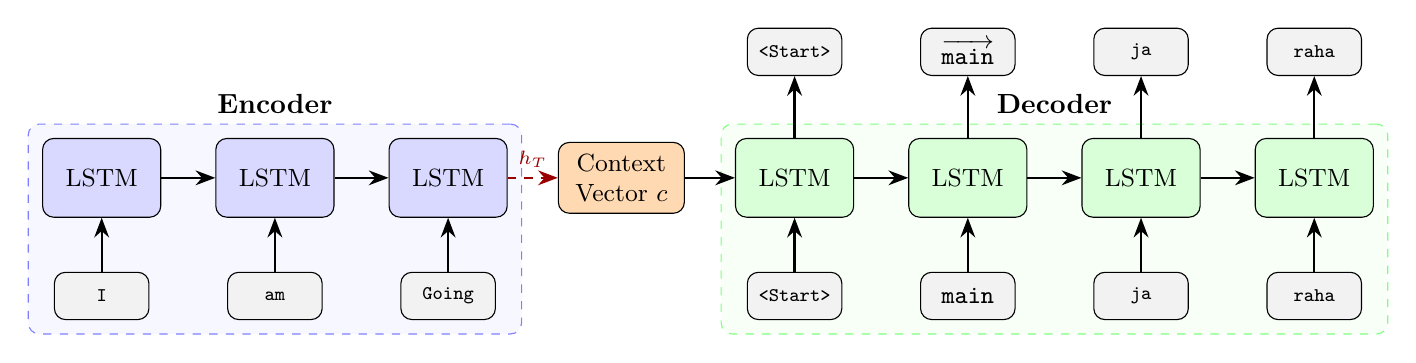
\begin{tikzpicture}[
  cell/.style={draw,rectangle,rounded corners,minimum width=1.5cm,minimum height=1.0cm,
               fill=blue!15,font=\small,align=center},
  dcell/.style={draw,rectangle,rounded corners,minimum width=1.5cm,minimum height=1.0cm,
                fill=green!15,font=\small,align=center},
  tok/.style={draw,rounded corners,minimum width=1.2cm,minimum height=0.6cm,fill=gray!10,font=\scriptsize},
  arr/.style={-{Stealth[length=2.5mm]},thick},
  darr/.style={-{Stealth[length=2.5mm]},thick,dashed,color=red!60!black}
]

% Encoder cells
\node[cell] (e1) at (0,0) {LSTM};
\node[cell] (e2) at (2.2,0) {LSTM};
\node[cell] (e3) at (4.4,0) {LSTM};

% Encoder arrows
\draw[arr] (e1) -- (e2);
\draw[arr] (e2) -- (e3);

% Encoder inputs
\node[tok] (i1) at (0,-1.5) {\texttt{I}};
\node[tok] (i2) at (2.2,-1.5) {\texttt{am}};
\node[tok] (i3) at (4.4,-1.5) {\texttt{Going}};
\draw[arr] (i1) -- (e1);
\draw[arr] (i2) -- (e2);
\draw[arr] (i3) -- (e3);

% Context vector
\node[draw,rectangle,rounded corners,minimum width=1.6cm,minimum height=0.9cm,
      fill=orange!30,font=\small,align=center] (ctx) at (6.6,0) {Context\\Vector $c$};
\draw[darr] (e3) -- (ctx) node[midway,above,font=\scriptsize]{$h_T$};

% Decoder cells
\node[dcell] (d0) at (8.8,0) {LSTM};
\node[dcell] (d1) at (11.0,0) {LSTM};
\node[dcell] (d2) at (13.2,0) {LSTM};
\node[dcell] (d3) at (15.4,0) {LSTM};

% Decoder arrows
\draw[arr] (ctx) -- (d0);
\draw[arr] (d0) -- (d1);
\draw[arr] (d1) -- (d2);
\draw[arr] (d2) -- (d3);

% Decoder outputs
\node[tok] (o0) at (8.8,1.6) {\texttt{<Start>}};
\node[tok] (o1) at (11.0,1.6) {\small\texttt{$\,\overrightarrow{\text{main}}\,$}};
\node[tok] (o2) at (13.2,1.6) {\texttt{ja}};
\node[tok] (o3) at (15.4,1.6) {\texttt{raha}};

% Decoder inputs (shifted teacher-forcing style)
\node[tok] (di1) at (8.8,-1.5) {\texttt{<Start>}};
\node[tok] (di2) at (11.0,-1.5) {\small\texttt{main}};
\node[tok] (di3) at (13.2,-1.5) {\texttt{ja}};
\node[tok] (di4) at (15.4,-1.5) {\texttt{raha}};

\draw[arr] (di1) -- (d0);
\draw[arr] (di2) -- (d1);
\draw[arr] (di3) -- (d2);
\draw[arr] (di4) -- (d3);
\draw[arr] (d0) -- (o0);
\draw[arr] (d1) -- (o1);
\draw[arr] (d2) -- (o2);
\draw[arr] (d3) -- (o3);

% Bounding boxes
\begin{scope}[on background layer]
  \node[draw=blue!50,dashed,rounded corners,fit=(e1)(e2)(e3)(i1)(i2)(i3),
        label=above:{\textbf{Encoder}},inner sep=5pt,fill=blue!3] {};
  \node[draw=green!50,dashed,rounded corners,fit=(d0)(d1)(d2)(d3)(di1)(di2)(di3)(di4),
        label=above:{\textbf{Decoder}},inner sep=5pt,fill=green!3] {};
\end{scope}

\end{tikzpicture}
\caption{Seq2Seq model for English-to-Hindi translation. The encoder (blue) processes
``I am Going'' and compresses the sequence into a context vector $c$. The decoder (green)
generates the Hindi translation token by token, conditioned on $c$.}
\label{fig:seq2seq}
\end{figure}

\subsection{Mathematical Formulation}

\textbf{Encoder:}
\begin{align}
  h_t^{\text{enc}} &= \text{LSTM}(x_t,\, h_{t-1}^{\text{enc}}), \quad t = 1,\ldots,T, \\
  c &= h_T^{\text{enc}}.
  \label{eq:context_vector}
\end{align}

\textbf{Decoder:}
\begin{align}
  s_0 &= c, \\
  s_j &= \text{LSTM}(y_{j-1},\, s_{j-1}), \quad j = 1,\ldots,T', \\
  p(y_j \mid y_{<j},\, c) &= \text{softmax}(W_s\, s_j + b_s).
\end{align}

The objective is to maximise the conditional log-likelihood:
\begin{equation}
  \mathcal{L} = \sum_{j=1}^{T'} \log p(y_j \mid y_{<j},\, c).
  \label{eq:seq2seq_loss}
\end{equation}

\subsection{Challenges}

\begin{warningbox}[title=Fixed-Size Context Vector Bottleneck]
The entire input sequence is compressed into a single fixed-size vector $c$
(see \cref{eq:context_vector}). For very long sequences this creates an
\textbf{information bottleneck}: early tokens may be poorly represented in $c$
by the time the encoder finishes. This limitation motivated the development of
\textbf{attention mechanisms} (Bahdanau et al., 2015) and eventually
\textbf{Transformers} (Vaswani et al., 2017).
\end{warningbox}

\subsection{Significance for LLMs}

As stated in the lecture: ``LLM evolution starts with the Seq2Seq model.'' The key contributions of
Seq2Seq are:
\begin{enumerate}[label=\arabic*.]
  \item Demonstrated that a single neural architecture can handle \emph{variable-length} input and
        output sequences.
  \item Introduced the \emph{encoder--decoder} paradigm that underlies T5, BART, and many
        other modern models.
  \item Motivated attention mechanisms by exposing the bottleneck of a single context vector.
\end{enumerate}

%=============================================================
\section{Comparison Summary}
\label{sec:comparison}
%=============================================================

\subsection{RNN Family Progression}

The three architectures form a progression of increasing expressiveness:
\begin{enumerate}
  \item \textbf{Vanilla RNN}: simple but suffers from vanishing gradients. No gating.
  \item \textbf{GRU}: two gates, one state; good balance of expressiveness and efficiency.
  \item \textbf{LSTM}: three gates, two states; most expressive but most costly.
\end{enumerate}

\begin{keyinsight}[title=Practical Rule of Thumb]
Start with GRU for most sequence modelling tasks. Switch to LSTM if you observe the GRU is not
capturing very long-range dependencies adequately. If computation is severely constrained, consider
GRU; if accuracy is paramount and data is abundant, LSTM is worth the extra parameters.
\end{keyinsight}

\subsection{GRU Equations at a Glance}

\begin{equation}
  \underbrace{z_t = \sigma(W_z[h_{t-1}, x_t])}_{\text{update gate}}
  \qquad
  \underbrace{r_t = \sigma(W_r[h_{t-1}, x_t])}_{\text{reset gate}}
\end{equation}
\begin{equation}
  \underbrace{\tilde{h}_t = \tanh(W[r_t\odot h_{t-1},\, x_t])}_{\text{candidate hidden state}}
\end{equation}
\begin{equation}
  \underbrace{h_t = (1-z_t)\odot h_{t-1} + z_t\odot\tilde{h}_t}_{\text{final hidden state (convex combination)}}
\end{equation}

%=============================================================
\section{Session Summary}
\label{sec:summary}
%=============================================================

Session~21 covered the following topics:

\begin{enumerate}[label=\S\arabic*.]
  \item \textbf{GRU overview}: GRU as a simplified LSTM with 1 state ($h_t$) and 2 gates
        ($r_t$, $z_t$), reducing from 4 sub-networks to 3, and from 2 state lines to 1.

  \item \textbf{Intuition}: The reset gate controls how much of the old memory is visible when
        computing the candidate; the update gate performs a smooth interpolation between old
        and new memory.

  \item \textbf{Mathematical flow}: Four equations -- update gate, reset gate, candidate hidden
        state, and final hidden state -- were derived and related to their LSTM counterparts.

  \item \textbf{Numerical walkthrough}: A 4-dimensional example was computed step by step,
        confirming the final state $h_t = [0.45, 0.74, -0.21, 0.68]^\top$ via the linear
        interpolation formula.

  \item \textbf{Gate correspondence}: GRU's reset gate $\equiv$ LSTM forget gate;
        $(1-z_t)$ $\equiv$ LSTM input gate; $z_t$ $\equiv$ LSTM output gate.

  \item \textbf{Seq2Seq introduction}: Encoder--decoder architecture using LSTM cells;
        the encoder compresses the input to a context vector $c = h_T^{\text{enc}}$, and the
        decoder generates a variable-length output sequence conditioned on $c$. Identified as
        the foundational architecture for modern LLMs.
\end{enumerate}

\subsection{Key Formulas}

\begin{align*}
  z_t &= \sigma(W_z\cdot[h_{t-1},x_t]) & \text{(update gate)}\\
  r_t &= \sigma(W_r\cdot[h_{t-1},x_t]) & \text{(reset gate)}\\
  \tilde{h}_t &= \tanh(W\cdot[r_t\odot h_{t-1},x_t]) & \text{(candidate)}\\
  h_t &= (1-z_t)\odot h_{t-1} + z_t\odot\tilde{h}_t & \text{(final state)}\\
  c &= h_T^{\text{enc}} & \text{(context vector)}
\end{align*}

\subsection{Looking Ahead}

The Seq2Seq model's fixed-size bottleneck motivates the introduction of the
\textbf{attention mechanism}: instead of using only the final encoder state $h_T$, the decoder
attends to all encoder hidden states $\{h_1, h_2, \ldots, h_T\}$ at each decoding step.
Attention is a prerequisite for understanding the Transformer architecture studied in later sessions.

\end{document}
